%% ------------------------------------------------------------------------- %%
\chapter{Hash Functions}
\label{cap:Hash Functions}

%% ------------------------------------------------------------------- %%
%\begin{itemize}
%\item Define Hash Function
%\item Give some examples of hash functions (Multiplicative / Remainder)
%\item Present Dragon Book metric and Evaluate hash functions
%\end{itemize}
%% ------------------------------------------------------------------- %%

Outside computer science, the word \textit{``hash''} in the english language means to ``chop'' or to ``mix'' something. This meaning is entirely related to what hash functions are supposed to do. hash functions are functions that are used to map data of an arbitrary size to data of a fized size \cite{HashFuncWiki}.

They have wide applications in computer science, being used in information and data scurity, compilers, distributed systems and hardcore algorithms. During this chapter I first define and explain the basics of a hash function, then I give an intiution in some metrics of what is a good hash function, as discussed in the famous \textit{``Red Dragon Book''} \cite{DragonBook} along with some reproduction of known results in the area.

The value extracted from the hash function for an object is usually called \textit{Hash Value}. The hash value is usually, but not necessarily, smaller than the object that generated it. For example, we can have a hash function that takes Gigabytes or Terabytes files and return an 8 bytes hash value.

\begin{figure}[h!]
  \centering
  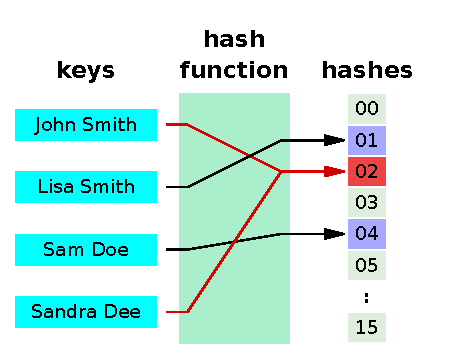
\includegraphics[width=10cm]{figuras/hash-function.pdf}
  \caption{Example of a hash function from string to 4 bit integer. }
\end{figure}

\bigskip

To formalize a little, lets define a hash function as a function \( H \) that takes an element \( x \in X \) and has \( [0, M) \) as a codomain.

This is the same definition used by Donald Knuth \cite{TAOCP3} and some articles \cite{RobinHoodHashing}. This definition makes sense for our case because we will be talking mostly about hash functions used in hash tables, and in that case we want integers that will be indexes in an array (as we will se later on). In other cases will may see hash functions value as strings, like for when we hash an string for password storage or when we use a hash function in files for check-sum (for when we are checking if two files are the same). For the goal of this thesis we will not be focusing on those functions, but it is important to notice that strings can also be abstracted to integers if we just look at the bytes.

For our specific case we are looking at a hash function that is good for the construction of hash tables, that is that is fast to calculate and minimizes the number of collisions. Depending on our goals we might want a different metric, for check-sums for example we may want a function that is very sensible to chages, and for passwords one that is very hard to find its inverse.

As said in Donald Knuth's book, we know that it is theoricatically impossible to create a hash functio that generates true random data from non random data in actual file, but we can do pretty close to that (or in some cases, even better).  Donald Knuth describes 2 specific methods for simple hash function, named \textit{division hashing} and \textit{multiplicative hashing} techniques. As the name sugests, the first is based on division and the former on multiplication.

The divison hashing method simply to represent the data as a number take the remainder of that number modulo a value. Supposing that we can represent the data as a non negative integer \( X \) the division hashing would be to choose a value M and the hashing function would be \( X mod M \). The C++11 code would look as following:

\begin{lstlisting}
unsigned_int divisionHashing(unsigned_int X, unsigned_int M) {
  return X % M;
}
\end{lstlisting}

In general large prime numbers tend to be a good value to \( M \), because if not we may have repetitions. One great example of this is if \( M \) is even, then the parity of hash value of \( X \) will match the parity of \( X \) (which will cause a bad distribution). The same pattern will happen in different intervals for different powers of \( 2 \).

For the multiplicative hashing, we can furst imagine that the overflow is like a ``natural'' modulo operation (We also have methods to take the modulo without overflowing, to know more about that ). Supposing that we can represent the data as an non negative integer \( X \), the multiplication hashing would be to choose a value \( A \) that we mulitply by \( X \) and then take the value module \( M \) (That \( M \) is described as a power of \( 2 \) by Donald Knuth, so it would be a more ``General'' multiplicative method). The C++11 code would look as follwing:

\medskip

\begin{lstlisting}
unsigned_int multiplicativeHashing(unsigned_int X,
                                   unsigned_int A,
                                   unsigned_int M) {
  return (A * X) % M; 
}
\end{lstlisting}

As you can see from above multiplicative hashing is just a more general division hashing. In knuth's book he restricts \( A \) to be relatively prime to \( w \), being \( w \) the size of a ``word'' in the machine (which is \( MAX\_INT \) in our case). That definition is often useful if you can retrieve a value \( Y \) for a given hahs value \( F \). It is good to note here that if \( H(X) = F \) and \( H(Y) = F \), \( X \) is not necessarily equal to \( Y \), as two keys can have the same hash value.

Here it is good to note, we have many ways of converting non numerical data to non negative integers. In the end, it is all just a sequence bytes, that when readed in a specific way form another type of data, such as images or strings. For example, one way of transforming a string to a non negative integer is summing the ASCII value of its characters. The C++11 code for that would look as following:

\begin{lstlisting}
unsigned_int convertStringToInteger(string str) {
  unsigned_int hashValue = 0;
  for (char c : str) {
    hashValue += (int) c;
  }
  return hashValue;
}
\end{lstlisting}

We always use usigned integers for our non negative integer calculations due to the natural modulo operation of it on overflow cases. It is equivalent to having a \( mod 2^{32} \) every time it overflows (As we only look at the leading 32 bits).